\newpage
\section{Example 4: Gap detection in child mode}

\subsection{General description of the experiment}
See \filename{examples/manual/gapdetectionchild.apx}. This is an
example of a gap detection task adapted to the interest of
children: two stimuli are presented to the listener in random
order, a stationary noise and an interrupted noise. It is the same
experiment as example 3, but pictures (movies) of cars replace
buttons on the screen, and a smiley panel is
shown(figure~\ref{fig:gapchild}). During the presentation of
stimuli the cars are animated. The child's task is to indicate the
stimulus with the interruption. Feedback is provided by smileys
and the minimal detectable gap is determined by means of an
adaptive procedure (here 2-down, 1-up). Only those elements that
are specific to the child mode are described in this example.

\index{Example: gap detection - child mode}

\begin{figure}
 \centering
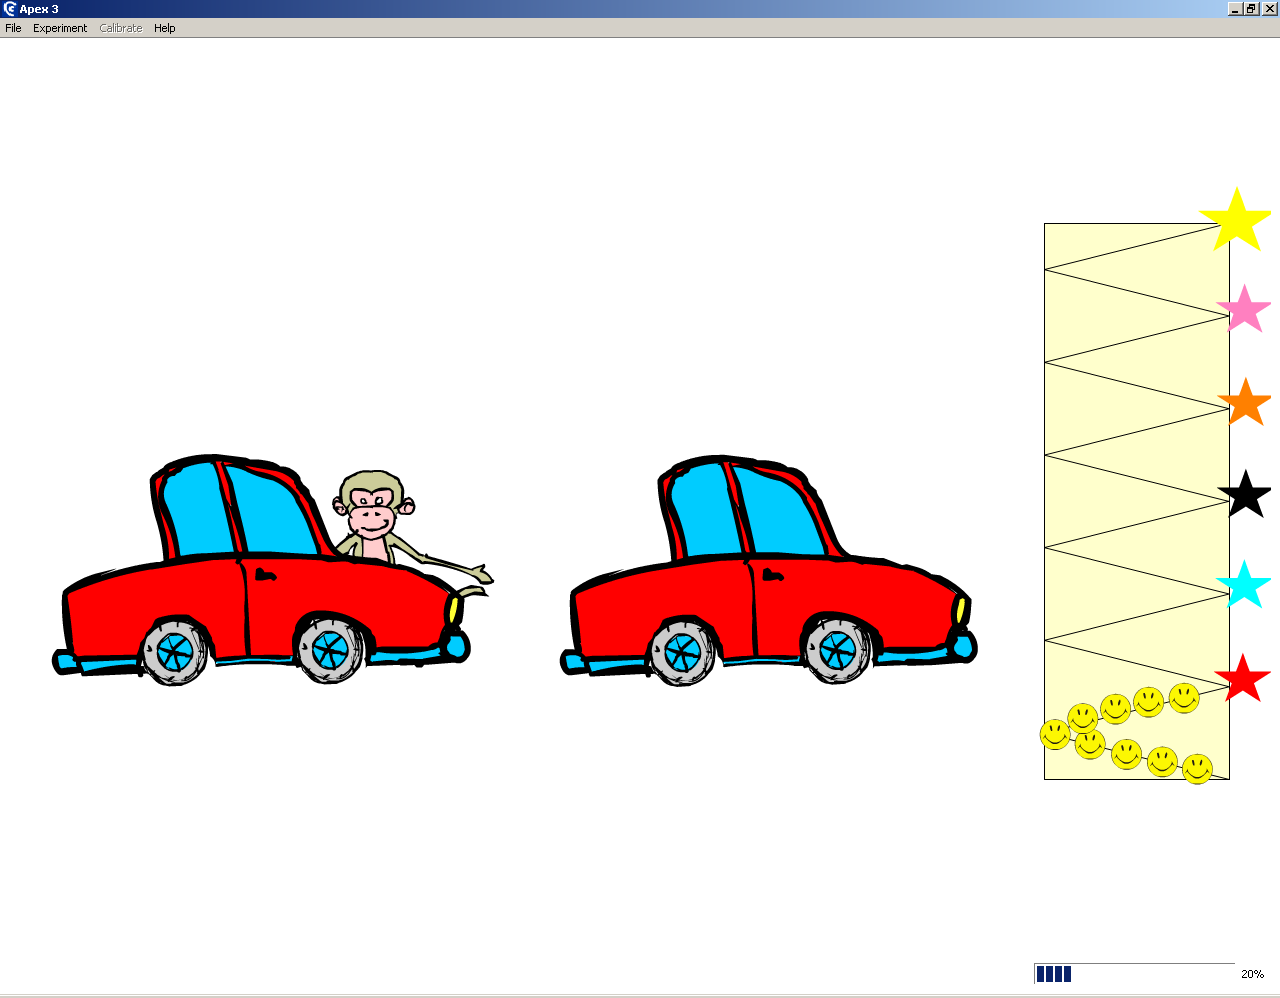
\includegraphics[width=\textwidth]{example4gapdetectionchild.png}
 \caption{Example of gap detection in child mode}
 \label{fig:gapchild}
\end{figure}

\subsection{Conceptual}
The main concepts illustrated in this example are
\textbf{childmode}, and \textbf{reinforcement}. Child mode
involves a different panel, and intro/outro movies.

\subsection{Detailed description of various elements}

\begin{lstlisting}
<screens>
    <uri_prefix>car/</uri_prefix>
    <general>
      <showpanel>true</showpanel>
    </general>
    <reinforcement>
      <progressbar>true</progressbar>
      <feedback length="300">true</feedback>
      <showcurrent>true</showcurrent>
    </reinforcement>
    <childmode>
      <panel>reinforcement.swf</panel>
    </childmode>
    <screen id="screen1">
      <gridLayout height="1" width="2" id="main_layout">
        <flash row="1" col="1" id="button1">
          <path>stillcar.swf</path>
          <feedback>
            <highlight>rijden.swf</highlight>
            <positive>goodcar.swf</positive>
            <negative>badcar.swf</negative>
          </feedback>
        </flash>

        <flash row="1" col="2" id="button2">
          <path>stillcar.swf</path>
          <feedback>
            <highlight>rijden.swf</highlight>
            <positive>goodcar.swf</positive>
            <negative>badcar.swf</negative>
          </feedback>
        </flash>
      </gridLayout>

      <buttongroup id="buttongroup1">
        <button id="button1"/>
        <button id="button2"/>
      </buttongroup>
      <default_answer_element>buttongroup1</default_answer_element>
    </screen>
  </screens>
\end{lstlisting}

\element{screens}

\begin{itemize}
\item \element{uri_prefix} a relative path is specified here
(relative with respect to the experiment file). This only applies
to the movies in \element{screen}. There are 3 ways to specify a
prefix: by directly specifying an absolute path, by directly
specifying a path relative to the experiment file or by referring
to a prefix stored in \filename{apexconfig.xml}. Please refer to
section~\ref{sec:prefixes} for more information.

\item \element{general}

\begin{itemize}

\item \element{show panel} if \xml {true} a panel will be shown
with smileys (see figure \textbf{presented above})

\end{itemize}

\item \element{reinforcement}
\begin{itemize}
\item \element{progressbar} If \xml {true} a progress bar will be
displayed on the right hand side with smileys. The progress bar
shows when a reversal occurs in an adaptive procedure (while the
number of trials varies).

\item \element{feedback length} duration of the time after
response (in msec) that \apex waits before presenting the next
trial. During this interval feedback can be displayed

\item \element{showcurrent} the interval is highlighted while a
signal is presented

\end{itemize}

\item\element{childmode} replaces the ``standard'' panel, sets
some defaults, enables intro/outro movies and changes the
background colour

\begin{itemize}

\item \element{panel} the name of the movie file, per frame
(smileys and panel are a collection of frames)

\end{itemize}

\end{itemize}

\element{screen} Each screen has an ID by which it can be referred
to elsewhere in the experiment. In this example the screen
displays two movies, each containing a car.

\begin{itemize}
\item \element{gridlayout} places elements in an irregular grid.
The screen is divided into sections according to the values. In
this example there are equal number of rows and columns.

\begin{itemize}
\item \element{flash} replaces \element{button} of the standard
version

\begin{itemize}
\item \element{path} the name of the flash movie file on disk,
when there is no animation.

\item \element{feedback}


\item \element{highlight}the name of the file while the car moves

\item \element{positive} the name of the movie file following a
correct response (here a monkey waving)

\item \element{negative} the name of the movie file following an
incorrect response  (the trunk of an elephant)

\end{itemize}

\end{itemize}

\item \element{buttongroup} defines a group of screen elements
(those that are displayed on the screen). As many elements can be
defined in a screen, \apex has no way to know which element
contains the subject's response. Therefore, in
\element{default_answer_element} the element is designated that
contains the subject's response. In the case of screen elements
that are clicked in order to respond, the example is further
complicated by the fact that we cannot specify just one of the
elements (buttons, pictures), but that the response rather comes
from a group of elements. This is when a \element{buttongroup} can
be used to group together different screen elements.


\end{itemize}
\index{screens}

\index{uri prefix}

\index{general}

\index{show panel}

\index{reinforcement}

\index{progressbar}

\index{feedback length}

\index{showcurrent}

\index{childmode}

\index{panel}

\index{screen}

\index{gridlayout}

\index{flash row}

\index{path}

\index{feedback}

\index{highlight}

\index{positive}

\index{negative}

\index{button}

\index{buttongroup}

\index{default answer element}
